\documentclass{beamer}
% imprimir
% \documentclass[handout]{beamer} 
% \usepackage{pgfpages}
% \pgfpagesuselayout{4 on 1}[a4paper,landscape,border shrink=5mm]

\mode<presentation> {
  \usetheme{Warsaw}
  \setbeamercovered{transparent}
}

\usebackgroundtemplate{
\includegraphics[width=\paperwidth]{figs/libresoft-bg.png}}

\usepackage[spanish]{babel}
\usepackage[utf8]{inputenc}
\usepackage{graphics}
\usepackage{amssymb} % Simbolos matematicos

%% Metadatos del PDF.
\hypersetup{
  pdftitle={Presentación del curso},
  pdfauthor={Jose Castro, Miguel Vidal},
  pdfcreator={GSyC/Libresoft, Universidad Rey Juan Carlos},
  pdfproducer=PDFLaTeX,
  pdfsubject={Master on libre software - 2010/2011},
}

% Inicio de la presentación
\begin{document}

% Metadatos de la presentacion
\title{Libre Software on Servers}
\subtitle{Master on libre software - 2010/2011} 
%\url{http://master.libresoft.es}
%}
\institute{\{jfcastro,mvidal\}@libresoft.es}
\author{Jose Castro, Miguel Vidal}
\date{April 1, 2011}

% Cover slide
\frame{
  \maketitle
  \begin{center}
    
\includegraphics[width=6cm]{figs/gsyc-urjc}
  \end{center}
}

%% License slide
\begin{frame}
  \vspace{3cm}
  \begin{flushright}
    {\footnotesize \copyright{2011} Jose Castro, Miguel Vidal.} \\
    \vspace{0.25cm}
    {\scriptsize Algunos derechos reservados. \\
    Presentación distribuida bajo licencia Creative Commons Reconocimiento 3.0 España}\\
    \vspace{0.25cm}
  \end{flushright}
  \begin{center}
    \href{http://creativecommons.org/licenses/by/3.0/es}{
\includegraphics[width=2cm]{figs/cc-by.png}} \\
    {\tiny \url{http://creativecommons.org/licenses/by/3.0/es}}
  \end{center}
\end{frame}


\section{Operating systems}
%%%%%%%%%%%%%%%%

\begin{frame}
  \frametitle{Operating systems}
  \begin{center}
    \Huge Operating systems
  \end{center}
\end{frame}

\begin{frame}
  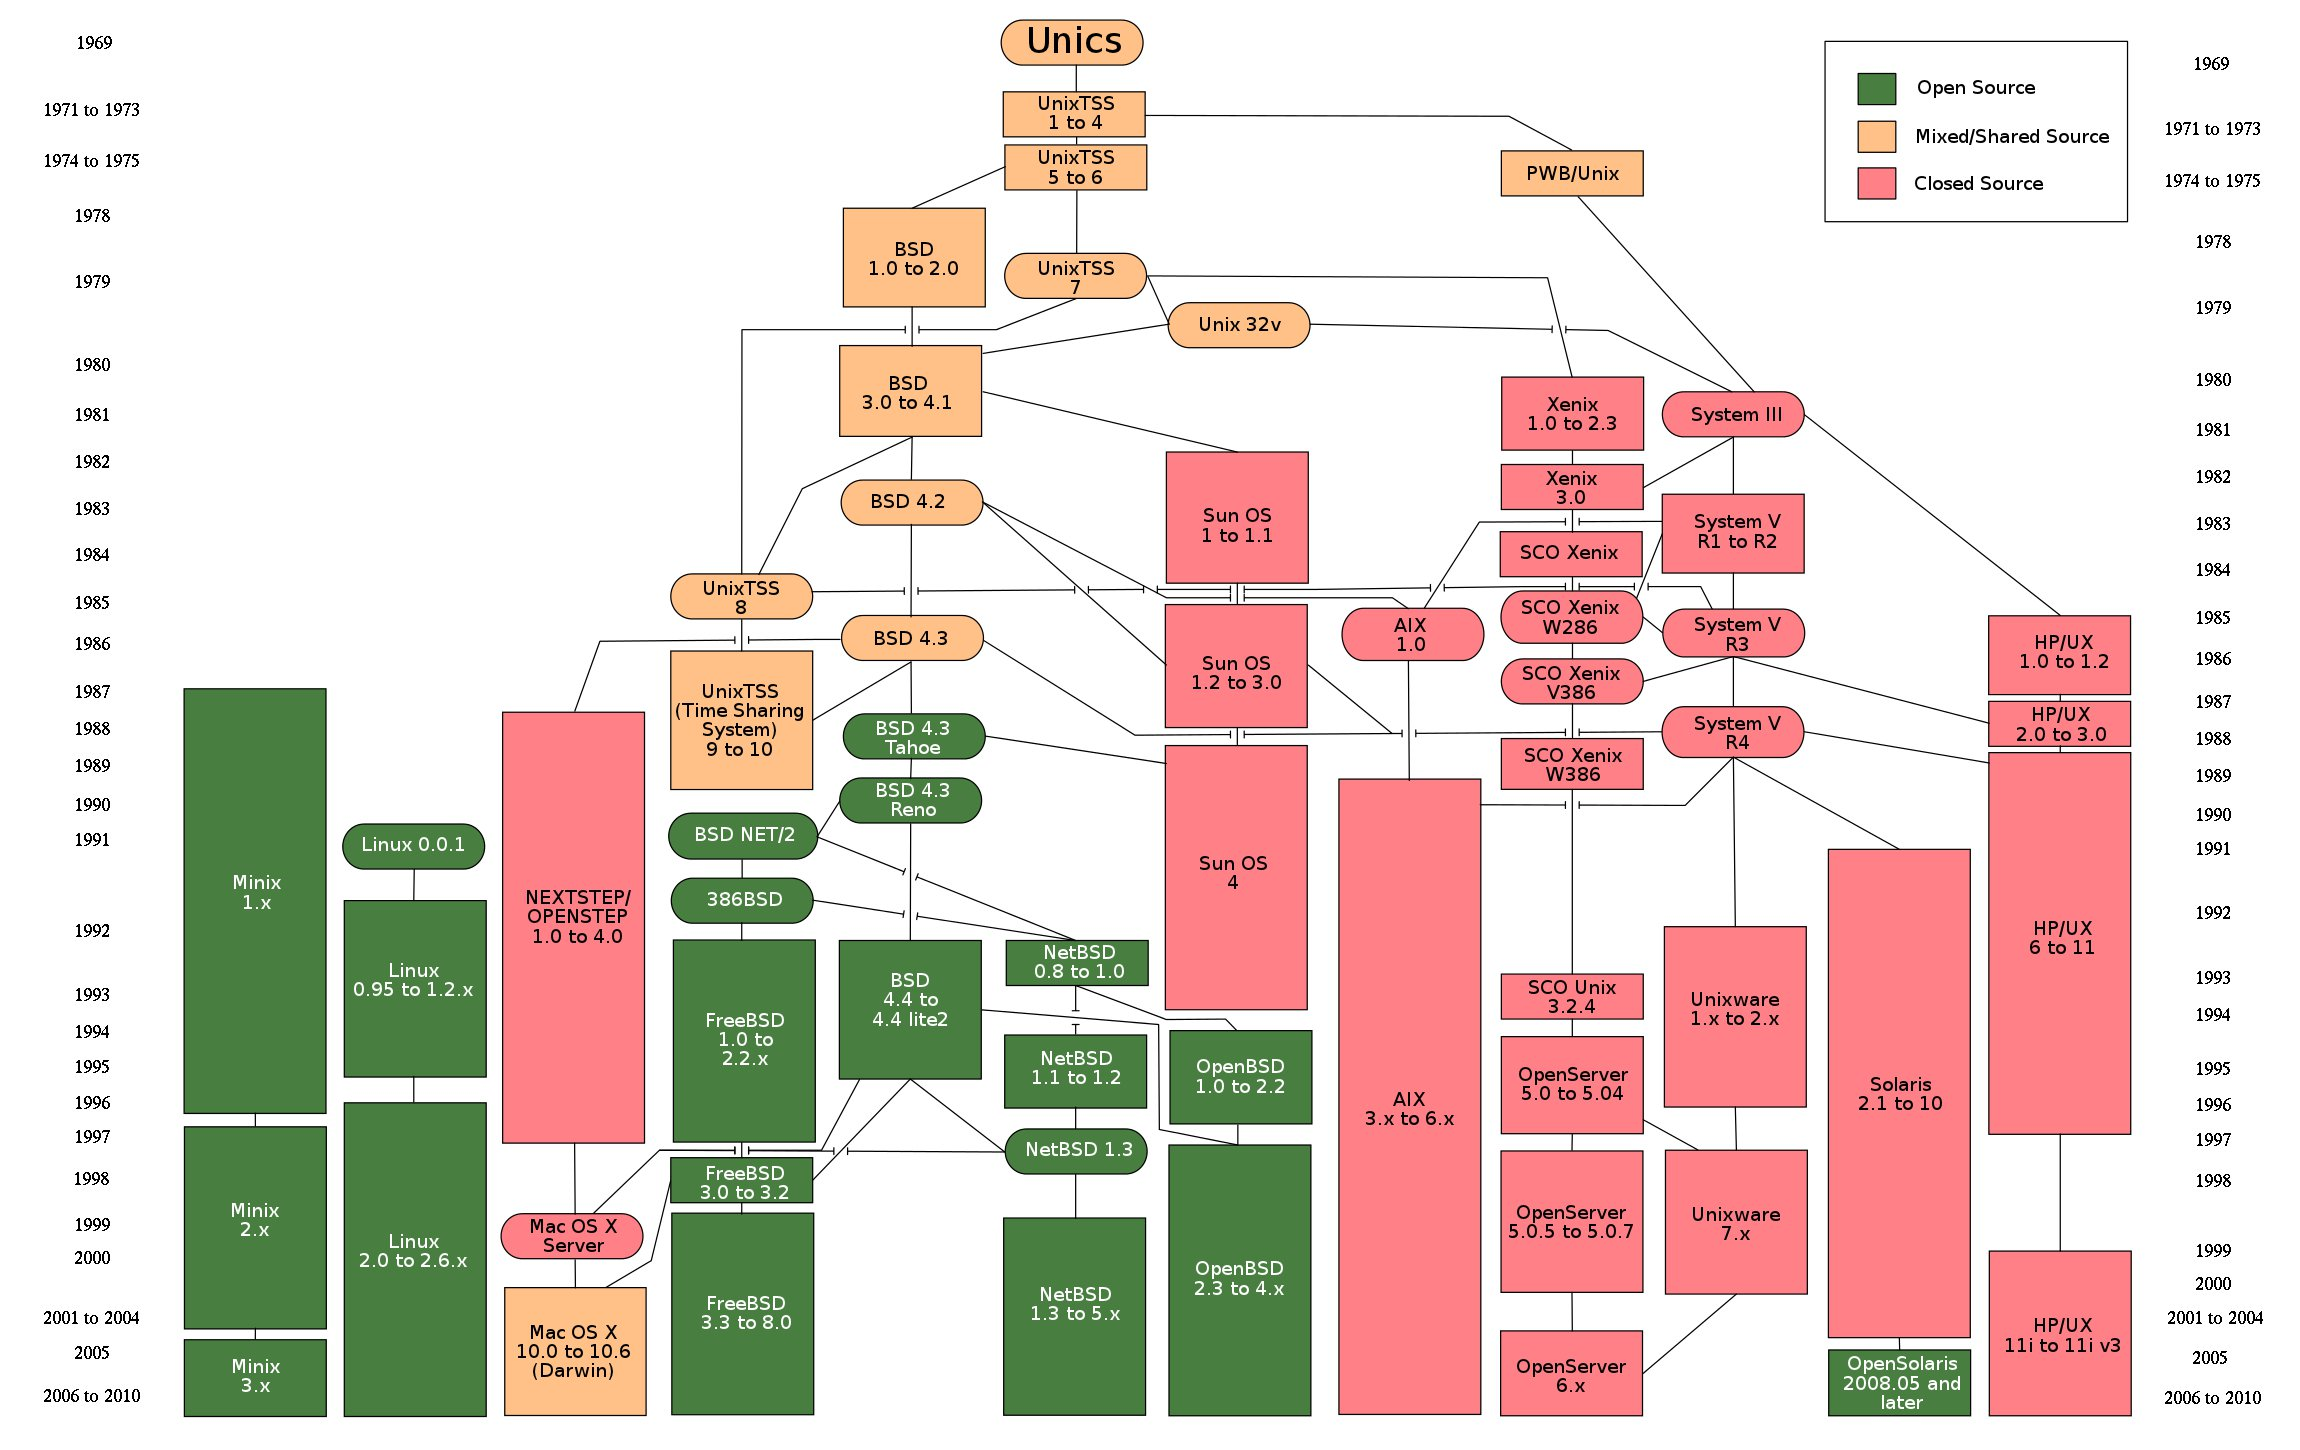
\includegraphics[width=10cm]{figs/Unix_history-simple.jpg}
\end{frame}
  \subsection{Linux}
  \begin{frame}
    \frametitle{Linux}
    \textbf{Linux}
    \begin{itemize}
      \item Linus Torvald in 1991 (and just for fun)
      \item From scratch
      \item Very software from BSD
      \item GPLv2 license
      \item Bazaar model: release early, release often
      \item March 1994: version 1.0
      \item A lot of distributions 
    \end{itemize}
  \end{frame}
  
  \subsection{OpenBSD}
  \begin{frame}
    \frametitle{OpenBSD}
    \textbf{OpenBSD}
    \begin{itemize}
      \item Focused on security and freedom
      \item Simplicity and stability (not cool)
      \item Best tools: \textit{OpenSSH} and \textit{PF}
      \item Very usefull documentation
      \item CVS and commits
    \end{itemize}
  \end{frame}
  
  \subsection{FreeBSD and NetBSD}
  \begin{frame}
    \frametitle{FreeBSD and NetBSD}
    \textbf{FreeBSD}
    \begin{itemize}
      \item The most popular BSD systems
      \item Good choice for desktop
      \item Operating systems level virtualization: \textit{jails}
      \item ZFS ported since 7.0
    \end{itemize}
    \textbf{NetBSD}
    \begin{itemize}
      \item Focused on portability (more than 56 architectures)
      \item Predecessor of OpenBSD
    \end{itemize}
  \end{frame}
  
  \subsection{illumos / OpenIndiana}
  \begin{frame}
    \frametitle{illumos / OpenIndiana}
    \textbf{illumos / OpenIndiana}
    \begin{itemize}
      \item OpenSolaris fork
      \item Leadered by Garret D'amore (Nexenta)
      \item Features inherited:
        \begin{itemize}
          \item SMF: Service Manager Facility
          \item ZFS: Zettabyte File System
          \item DTrace: debug tool at real time without performance impact
        \end{itemize}
      \item OpenIndiana was first distribution based on illumos
    \end{itemize}
  \end{frame}


\section{Internet Servers}
%%%%%%%%%%%%%%%

\begin{frame}
  \frametitle{Internet Servers}
  \begin{center}
    \Huge Internet Servers
  \end{center}
\end{frame}

  \subsection{Web}
  \begin{frame}
    \frametitle{Web -- Apache and Cherokee}
    \textbf{Apache}
    \begin{itemize}
      \item The most widely used web server
      \item Apache license
      \item Modules: proxies, dav (svn and webdav), ACLs...
    \end{itemize}
    \textbf{Cherokee}
    \begin{itemize}
      \item Very fast, flexible and easy to configure.
      \item GPLv2 license
      \item Cherokee Market: first wep-app Marketplace
    \end{itemize}
  \end{frame}

  \subsection{Mail}
%  http://en.wikipedia.org/wiki/Comparison_of_mail_servers
% http://www.securityspace.com/s_survey/data/man.200707/mxsurvey.html
  
  \begin{frame}
    \frametitle{Mail -- sendmail and qmail}
    \textbf{sendmail}
    \begin{itemize}
      \item Very knowed in free software and Unix communities
      \item Difficult configuration: all configurations into a file
    \end{itemize}
    \textbf{qmail}
    \begin{itemize}
      \item Safe replacement of sendmail by Daniel J. Bernstein
      \item Included Maildir format (a file, a message)
      \item Features: security, performance, simplicity, modularity
      \item Last version of 1998
      \item Public domain
    \end{itemize}
  \end{frame}
  
  \begin{frame}
    \frametitle{Mail -- Exim and Postfix}
    \textbf{Exim}
    \begin{itemize}
      \item EXperimental Internet Mailer
      \item University of Cambridge Computing Service's e-mail systems
      \item GPLv3 license
      \item Por defecto en los sistemas Debian y derivados
      \item Debian systems and derivates by default
      \item Monolithic: only a binary for all (less secure)
    \end{itemize}
    \textbf{Postfix}
    \begin{itemize}
      \item Also known as VMailer and IBM Secure Mailer
      \item IBM Public license (copyleft)
      \item Fast and easier-to-administer focused
      \item Differents daemons for differents proposals
    \end{itemize}
  \end{frame}
  
  \subsection{Mailing lists}
  \begin{frame}
    \frametitle{Mailing lists -- Mailman}
    \textbf{Mailman}
    \begin{itemize}
      \item GNU project. GPLv3 license
      \item Coded in python
      \item Web interface for administration, archive lists, spam filtering
      \item Since 1999. Replacement to Majordomo
    \end{itemize}
  \end{frame}
  
  \begin{frame}
    \frametitle{Mailing lists -- SmartList and ezmlm}
    \textbf{SmartList}
    \begin{itemize}
      \item Procmail development team
      \item Requires Procmail to run
      \item GPL or Artistic License (1.0 no free, 2.0 free and compatible con GPL)
    \end{itemize}
    \textbf{ezmlm}
    \begin{itemize}
      \item Developed by Daniel J. Bernstein
      \item Public domain
      \item Only works with the qmail mail transfer agent
    \end{itemize}
  \end{frame}
  
  \subsection{DNS}
  \begin{frame}
    \frametitle{DNS -- bind and djbdns}
    \textbf{bind}
    \begin{itemize}
      \item Berkeley Internet Name Domain (aka named)
      \item BSD license
      \item University of California, Berkeley (UCB) in the early 1980s
      \item DLZ (Dynamically Loadable Zones) is a patch for BIND version 9 that simplifies BIND administration and reduces memory usage and startup time. 
    \end{itemize}
    \textbf{djbdns}
    \begin{itemize}
      \item Developed by Daniel J. Bernstein due to his frustrations with repeated BIND security hole
      \item Public domain
    \end{itemize}
  \end{frame}


\section{Sysadmin tools}
%%%%%%%%%%%%%%

\begin{frame}
  \frametitle{Sysadmin tools}
  \begin{center}
    \Huge Sysadmin tools
  \end{center}
\end{frame}

  \subsection{Monitorization}
  \begin{frame}
    \frametitle{Monitorization}
    \begin{itemize}
      \item Nagios
      \item Zabbix
      \item Pandora
      \item Osmius
    \end{itemize}
  \end{frame}
  
  \subsection{Directory}
  \begin{frame}
    \frametitle{Directory -- OpenLDAP}
    \textbf{OpenLDAP}
    \begin{itemize}
      \item Lightweight Directory Access Protocol implementation
      \item OpenLDAP Public License
      \item Several backend schemas and replication
    \end{itemize}
  \end{frame}

  \subsection{Backups}
  \begin{frame}
    \frametitle{Backups -- Amanda and Bacula}
    \textbf{Amanda}
    \begin{itemize}
      \item Advanced Maryland Automatic Network Disk Archiver
      \item Amanda Copyright and License (BSD-style license)
      \item Supports Windows systems using Samba
    \end{itemize}
    \textbf{Bacula}
    \begin{itemize}
      \item GPLv2 license
      \item Command line console, GUI or web interface
      \item Bacula is designed to be modular (director, storage, file, client)
      \item Bacula supports Linux, UNIX, Windows, and Mac OS X backup clients
    \end{itemize}
  \end{frame}


\section{Storage}
%%%%%%%%%

\begin{frame}
  \frametitle{Storage}
  \begin{center}
    \Huge Storage
  \end{center}
\end{frame}

  \subsection{SAMBA and NFS}
  \begin{frame}
    \frametitle{SAMBA and NFS}
    \textbf{SAMBA}
    \begin{itemize}
      \item Before SMB and now CIFS
      \item GPLv3 license
      \item File and print services
      \item Runs on most Unix and Unix-like systems
    \end{itemize}
    \textbf{NFS}
    \begin{itemize}
      \item Network file system
      \item Developed by Sun Microsystems in 1984
      \item NFSv4.1 adds the Parallel NFS (pNFS) capability
    \end{itemize}
  \end{frame}
  
  
  \subsection{ZFS}
  \begin{frame}
    \frametitle{ZFS}
    \textbf{ZFS}
    \begin{itemize}
      \item Zetabyte File System
      \item CDDL license
      \item Designed by Sun Microsystems from scratch
      \item For high storage capacities
      \item Important features:
        \begin{itemize}
          \item volume management, storage pools
          \item snapshots and copy-on-write clones
          \item RAID-Z and native NFS, CIFS and iSCSI
          \item transparent encryption and native compression
          \item deduplication
        \end{itemize}
      \item Easy administration
      \item Free alternative to NetApp
    \end{itemize}
  \end{frame}

  \subsection{drbd}
  \begin{frame}
    \frametitle{drbd}
    \textbf{drbd}
    \begin{itemize}
      \item Distributed Replicated Block Device
      \item Kernel module for Linux kernel
      \item GPLv2 license
      \item Normally used on high availability (HA) clusters
    \end{itemize}
  \end{frame}
  
  \subsection{FreeNAS}
  \begin{frame}
    \frametitle{FreeNAS}
    \textbf{FreeNAS}
    \begin{itemize}
      \item Distribution based on FreeBSD
      \item BSD license
      \item Network-attached storage server, supporting: CIFS (Samba), FTP, NFS, rsync, AFP protocols, iSCSI, S.M.A.R.T., local user authentication, and software RAID (0,1,5,Z)
      \item ZFS fully supported
      \item Web-based configuration interface (inherited from m0n0wall)
    \end{itemize}
  \end{frame}

  
\section{Firewalls}
%%%%%%%%%%

\begin{frame}
  \frametitle{Firewalls}
  \begin{center}
    \Huge Firewalls
  \end{center}
\end{frame}

  \subsection{iptables and IPFilter}
  \begin{frame}
    \frametitle{iptables and IPFilter}
    \textbf{iptables}
    \begin{itemize}
      \item Based in Netfilter (kernel module, user space tools and libraries)
      \item GPLv2 license
      \item Only for Linux
    \end{itemize}
    \textbf{IPFilter}
    \begin{itemize}
      \item Also known as ipf
      \item IPF-own licensing (allows redistribution of modified versions but prohibits relicensing)
      \item Delivered with FreeBSD, NetBSD, DragonFlyBSD and OpenSolaris/illumos 
    \end{itemize}
  \end{frame}
  
  
  \subsection{Packet Filter}
  \begin{frame}
    \frametitle{Packet Filter}
    \textbf{Packet Filter}
    \begin{itemize}
      \item Also known as pf
      \item Developed on OpenBSD (ported to many others operating systems)
      \item As a replacement for IPFilter due to desagree whit its license
    \end{itemize}
  \end{frame}

  \subsection{CARP and OpenBGPD}
  \begin{frame}
    \frametitle{CARP and OpenBGPD}
    \textbf{CARP}
    \begin{itemize}
      \item Common Address Redundancy Protocol
      \item Provide failover redundancy
      \item In some configurations CARP can also provide load balancing functionality
      \item It is a free, non patent-encumbered alternative to Cisco's HSRP
    \end{itemize}
    \textbf{OpenBGPD}
    \begin{itemize}
      \item Gateway Load Balancing Protocol implementation
      \item Exchange routes
      \item Developed by OpenBSD project (also allowed on FreeBSD)
      \item ISC license (BSD-style license)
    \end{itemize}
  \end{frame}
  
  \subsection{M0n0wall and PFSense}
  \begin{frame}
    \frametitle{M0n0wall and PFSense}
    \textbf{M0n0wall}
    \begin{itemize}
      \item Embedded firewall distribution of FreeBSD
      \item BSD license
      \item Can be put on Compact Flash
      \item Web-based interface
    \end{itemize}
    \textbf{PFSense}
    \begin{itemize}
      \item Firewall/router distribution based on a fork of the m0n0wall project
      \item BSD license
      \item Real Time Information
      \item Expansions: Squid proxy server and Snort intrusion prevention/detection system
      \item RRD Graphs Reporting
      \item Redundancy with CARP
    \end{itemize}
  \end{frame}


\section{Virtualization}
%%%%%%%%%%%%%

\begin{frame}
  \frametitle{Virtualization}
  \begin{center}
    \Huge Virtualization
  \end{center}
\end{frame}

  \subsection{Introduction}
  \begin{frame}
    \frametitle{What is}
    \begin{itemize}
      \item Hardware/software combination which giva a computer to act as several ones
      \item It includes making a single physical resource appear to function as multiple logical resources
      \item Virtualization is a methodology of dividin the resources of a computer into multiple execution enviroments
      \item Colloquially, virtualization refers to the abstraction of computer resources
    \end{itemize}
  \end{frame}
  
  \begin{frame}
    \frametitle{Hypervisors}
    \begin{itemize}
      \item The hypervisor abstracts the physical resources of the host computer into discrete ``virtual machines''
      \item We have two hypervisor classes:
        \begin{itemize}
          \item Type 1 (or native): hypervisor is a layer between hardware and all OS. Host OS is known as Control Domain
          \item Type 2 (or hosted): hypervisor is a software layer running over the host OS
        \end{itemize}
    \end{itemize}
  \end{frame}
  
  \begin{frame}
    \frametitle{Types of virtualization}
    \begin{itemize}
      \item Emulation: virtual machine simulates entire hardware
      \item Full virtualization: same as emulation but not different architecture
      \item Paravirtualization: hypervisor exports a modified version of the host
      \item Operating system-level virtualization: lightweight virtualization. No hypervisor.
    \end{itemize}
  \end{frame}
  
  
  \subsection{Xen and kvm}
  \begin{frame}
    \frametitle{Xen and kvm}
    \textbf{Xen}
    \begin{itemize}
      \item Xen uses paravirtualization. Guest operating system must be modified
      \item Also full virtualization with Intel VT and AMD-V
      \item Virtual machine migration, pause, restore, snapshot...
    \end{itemize}
    \textbf{kvm}
    \begin{itemize}
      \item Kernel-based Virtual Machine
      \item Linux kernel virtualization infraestructure
      \item First version included in Linux 2.6.20 (Feb 2007)
      \item \texttt{qemu} uses the \texttt{/dev/kvm} interface to setup VMs
    \end{itemize}
  \end{frame}
  
  \subsection{Solaris Zones and jails}
  \begin{frame}
    \frametitle{Solaris Zones and jails}
    \textbf{Solaris Zones}
    \begin{itemize}
      \item Operating system-level virtualization
      \item Global zone vs. local zones
      \item Provisioning and administration very simple
    \end{itemize}
    \textbf{jails}
    \begin{itemize}
      \item Operating system-level virtualization
      \item Security: easy isolation and easy delegation
      \item Since FreeBSD 4.0
    \end{itemize}
  \end{frame}
  
  \subsection{LDOMs}
  \begin{frame}
    \frametitle{LDOMs}
    \textbf{LDOMs}
    \begin{itemize}
      \item Full virtualization. Type 1 hypervisor based
      \item Requires special CPUs (Chip Multithreading = CMT)
      \item Each domain is a full virtual machine
      \item Operating system running inside Logical Domains can be managed independently
      \item But now, only SunOS is supported
    \end{itemize}
  \end{frame}
  
  \subsection{OpenVZ and Vserver}
  \begin{frame}
    \frametitle{OpenVZ and Vserver}
    \textbf{OpenVZ}
    \begin{itemize}
      \item Operating system-level virtualization 
      \item Technology based on the Linux kernel 
      \item GPLv2 license
      \item IPSec is not supportes inside containers
      \item Live migration not supported
    \end{itemize}
    \textbf{Linux Vserver}
    \begin{itemize}
      \item Operating system-level virtualization
      \item GPLv2 license
      \item Requires that the host kernel be patched
    \end{itemize}
  \end{frame}
  
  \subsection{Linux Containers}
  \begin{frame}
    \frametitle{Linux Containers}
    \textbf{Linux Containers}
    \begin{itemize}
      \item Also known as lxc
      \item It is mainline (submitted to and accepted by the linux official kernel tree)
      \item Based on \textit{cgroups} since version 2.6.29
    \end{itemize}
  \end{frame}


\section{High availabilty}
%%%%%%%%%%%%%

\begin{frame}
  \frametitle{High availability}
  \begin{center}
    \Huge High availability
  \end{center}
\end{frame}

  \subsection{Linux HA}
  \begin{frame}
    \frametitle{LinuxHA}
    \textbf{Linux HA}
    \begin{itemize}
      \item Build a cluster with Linux nodes
      \item Different schemas:
        \begin{itemize}
          \item active-pasive
          \item active-active
          \item N+1
          \item N-to-N
        \end{itemize}
      \item Proffesional cluster solution with \textit{drbd}
    \end{itemize}
  \end{frame}
  
  \subsection{OHAC}
  \begin{frame}
    \frametitle{OHAC}
    \textbf{OHAC}
    \begin{itemize}
      \item Open HA Cluster is descent of Solaris Cluster
      \item Synchronous and asynchronous replication
      \item \textit{quorum} software, fencing, IPSec, Crossbow...
      \item OpenSolaris and illumos
      \item Architectures: x86 and SPARC
    \end{itemize}
  \end{frame}


\section{Cloud Computing}
%%%%%%%%%%%%%%%

  \subsection{What is}
  \begin{frame}
    \frametitle{What is}
    \begin{itemize}
      \item Cloud Computing is not the same as virtualization management
      \item But most Cloud Computing deployments depend on virtualization
      \item Infraestructure capacity on CC is highly elastic (up or down)
      \item Clouds are hardware-based resources converted into a ``resource pool''
      \item IaaS, PaaS and SaaS. And autoprovisioning.
    \end{itemize}
  \end{frame}
  
  \subsection{OpenNebula}
  \begin{frame}
    \frametitle{OpenNebula}
    \textbf{OpenNebula}
    \begin{itemize}
      \item Developed by DSA-Research at UCM
      \item Apache license
      \item Toolkit to build any type of cloud: private, public and hybrid
      \item Sponsored by C12G Labs
      \item Is used by CERN, TID, hosting providers...
      \item Included in Debian Sid and Ubuntu
    \end{itemize}
  \end{frame}

% Cover slide
\frame{
  \maketitle
  \begin{center}
    
\includegraphics[width=6cm]{figs/gsyc-urjc}
  \end{center}
}
  
% Fin del documento
\end{document}
